\documentclass[border=20pt]{standalone}
\usepackage{tikz}
\usepackage[T1]{fontenc}

% Anthropic brand colors
\definecolor{clay}{HTML}{D97757}
\definecolor{sky}{HTML}{6A9BCC}
\definecolor{cactus}{HTML}{BCD1CA}
\definecolor{slate}{HTML}{141413}
\definecolor{ivory}{HTML}{FAF9F5}
\definecolor{fig}{HTML}{C46686}
\definecolor{olive}{HTML}{788C5D}
\definecolor{oat}{HTML}{E3DACC}
\definecolor{gray500}{HTML}{87867F}

\usetikzlibrary{positioning, calc}

\begin{document}
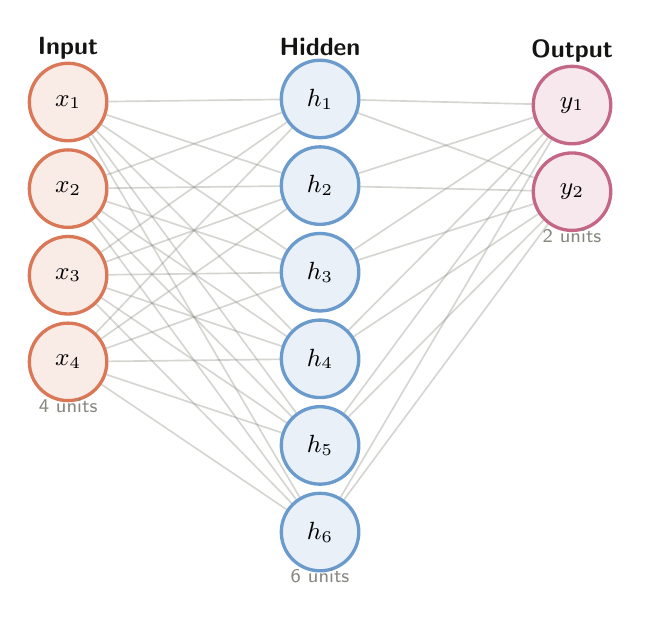
\begin{tikzpicture}[
    % Node styles
    input node/.style={
        circle,
        draw=clay,
        fill=clay!15,
        line width=1.2pt,
        minimum size=28pt,
        inner sep=0pt,
        font=\sffamily\small
    },
    hidden node/.style={
        circle,
        draw=sky,
        fill=sky!15,
        line width=1.2pt,
        minimum size=28pt,
        inner sep=0pt,
        font=\sffamily\small
    },
    output node/.style={
        circle,
        draw=fig,
        fill=fig!15,
        line width=1.2pt,
        minimum size=28pt,
        inner sep=0pt,
        font=\sffamily\small
    },
    connection/.style={
        draw=gray500,
        opacity=0.35,
        line width=0.6pt
    },
    layer label/.style={
        font=\sffamily\bfseries\small,
        text=slate
    }
]

% Layer spacing
\def\layersep{3.2cm}
\def\nodesep{1.1cm}

% Calculate vertical offsets for centering
% Hidden layer has 6 nodes -> spans 5*nodesep = 5.5cm, center at 2.75
% Input layer has 4 nodes -> spans 3*nodesep = 3.3cm, center at 1.65
% Output layer has 2 nodes -> spans 1*nodesep = 1.1cm, center at 0.55

\def\hiddenoffset{0}        % Reference layer (6 nodes)
\def\inputoffset{1.1}       % (6-4)/2 * nodesep = 1.1
\def\outputoffset{2.2}      % (6-2)/2 * nodesep = 2.2

% Input layer (4 nodes)
\foreach \i in {1,...,4} {
    \node[input node] (I-\i) at (0, -\i*\nodesep - \inputoffset) {$x_{\i}$};
}

% Hidden layer (6 nodes)
\foreach \i in {1,...,6} {
    \node[hidden node] (H-\i) at (\layersep, -\i*\nodesep - \hiddenoffset) {$h_{\i}$};
}

% Output layer (2 nodes)
\foreach \i in {1,...,2} {
    \node[output node] (O-\i) at (2*\layersep, -\i*\nodesep - \outputoffset) {$y_{\i}$};
}

% Connections: Input -> Hidden
\foreach \i in {1,...,4} {
    \foreach \j in {1,...,6} {
        \draw[connection] (I-\i) -- (H-\j);
    }
}

% Connections: Hidden -> Output
\foreach \i in {1,...,6} {
    \foreach \j in {1,...,2} {
        \draw[connection] (H-\i) -- (O-\j);
    }
}

% Layer labels
\node[layer label, above=12pt] at (0, -1*\nodesep - \inputoffset) {Input};
\node[layer label, above=12pt] at (\layersep, -1*\nodesep - \hiddenoffset) {Hidden};
\node[layer label, above=12pt] at (2*\layersep, -1*\nodesep - \outputoffset) {Output};

% Layer size annotations
\node[font=\sffamily\scriptsize, text=gray500, below=10pt] at (0, -4*\nodesep - \inputoffset) {4 units};
\node[font=\sffamily\scriptsize, text=gray500, below=10pt] at (\layersep, -6*\nodesep - \hiddenoffset) {6 units};
\node[font=\sffamily\scriptsize, text=gray500, below=10pt] at (2*\layersep, -2*\nodesep - \outputoffset) {2 units};

\end{tikzpicture}
\end{document}
